\subsection{Torsten Spis P{{\ae}}nt}
Torsten Spis P{\ae}nt is an original cartoon series in active development. It is about a young boy who is living with his mom in {\O}restaden, Copenhagen and his exploration of new and exciting food. In the pilot episode, Torsten's mom cites the old phrase "you are what you eat," and the gullible Torsten takes this as fact, letting his imagination bring him into the world of animated fruits and vegetables. \newline
As part of the publishing deal for Torsten Spis P{\ae}nt a series of accompanying games is required. The series is in early development and has yet to be greenlit. For this to happen, content needs to be presented and accepted. Part of this content is prototypes for future games, and that is where Triband enters the partnership. Triband made a series of very rough prototypes to explore different game mechanics. The best two were selected and the actual development of two prototypes were tasked to me and the other intern at Triband. The work was divided with the other intern producing the art and animation, and me the programming and implementation. The mechanics of the two prototypes were previously decided on so the amount of design work were limited.

\subsubsection{Madkamp}
Madkamp, or \textit{Food Fight}, is a game concept where the player is brought into Torsten's kitchen to, as the title suggest, fight with food. The player can look around the kitchen by utilising the mobile device's gyroscope and touch the screen to throw a random fruit or vegetable. \newline
Before starting the process we received some instructions on what the prototype had to contain:
\begin{itemize}
  \item Start screen including:
  \begin{itemize}
    \item Big play button
    \item Instructions button: Hit Torsten with the food. Raise the phone and look around to aim
  \end{itemize}
  \item End screen (appears after $\approx$45 seconds) including:
  \begin{itemize}
    \item Score: How many times you hit Torsten
    \item Play again button
  \end{itemize}
\end{itemize}
Additionally, a small model of the kitchen was made beforehand to better visualise the possibilities of the room (see figure \ref{kitchenmodel}).

\begin{center}
  \begin{figure}
    \noindent\makebox[\textwidth]{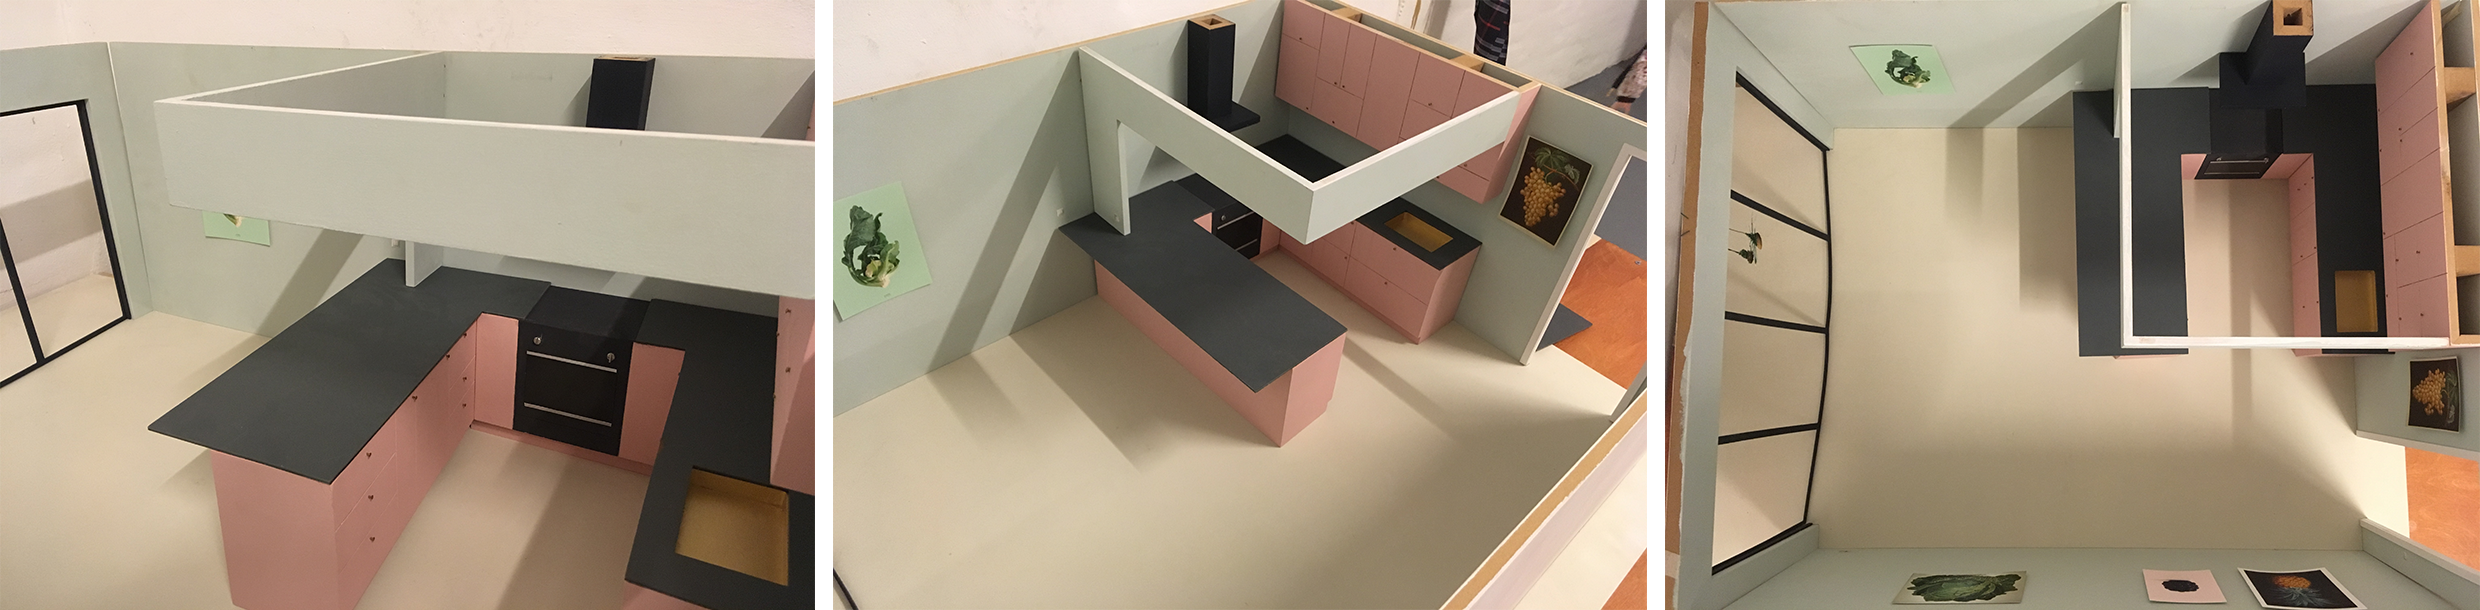
\includegraphics[width = \paperwidth]{Madkamp/KitchenModel}}
    \caption{A Model of Torsten's Kitchen}
    \label{kitchenmodel}
  \end{figure}
\end{center}

The work was then initiated with a division of labour. Art would be made by the other intern and implementation of controls and mechanics to me. I quickly set up a test level with some target practices to prototype the gyroscope and throwing controls (see figure \ref{TestScene}A). The gyroscopic input proved no difficulty but as I implemented the throwing mechanic I quickly realised that, to not confuse the player, the origin of all projectile needed to be centred on the screen and be projected in the orientation of the view. Originally, I wanted the player to be able to shoot from anywhere on the screen and shoot in the direction of the point in the game world the input was pointed at. Very quickly, however, this was deemed to be too complex for the target audience, so I chose to simplify the mechanic to the previously described mechanic.

Next challenge was visualising the point of impact for the projectiles in the form of splats. My first attempt at this was to simply spawn a sprite at the point of collision and rotate it according to the normal of the surface. For this to work the size of the sprite would have be adjusted according to the proximity of the closest edge of the surface. I accomplished this by stepping in four opposite directions iteratively and the first step that was not on the collision's surface determined the size of the sprite according to the distance between the collision point and the closest edge (see figure \ref{TestScene}B). The problem of this approach at visualising splats is that splats close to an edge will be miniscule, where a similar splat in the real world would instead wrap around the edge and continue on the next surface. Thinking that these splats were at the centre of what would make this game amusing, I scrapped this approach because I decided that it had no possibility of resulting in a satisfactory result. Instead I focused on an approach that utilised UV mapping \cite{mullen}. In brief, the 3D model that is capable of being hit by the projectiles has two UV maps: 1) On the top, a regular texture map. 2) On the bottom, a texture map with all surfaces covered in the splat material. Each time the model is hit, the surrounding area exposes the bottom layer with the splat material (see figure \ref{UVSplat}).

\begin{center}
  \begin{figure}
    \noindent\makebox[\textwidth]{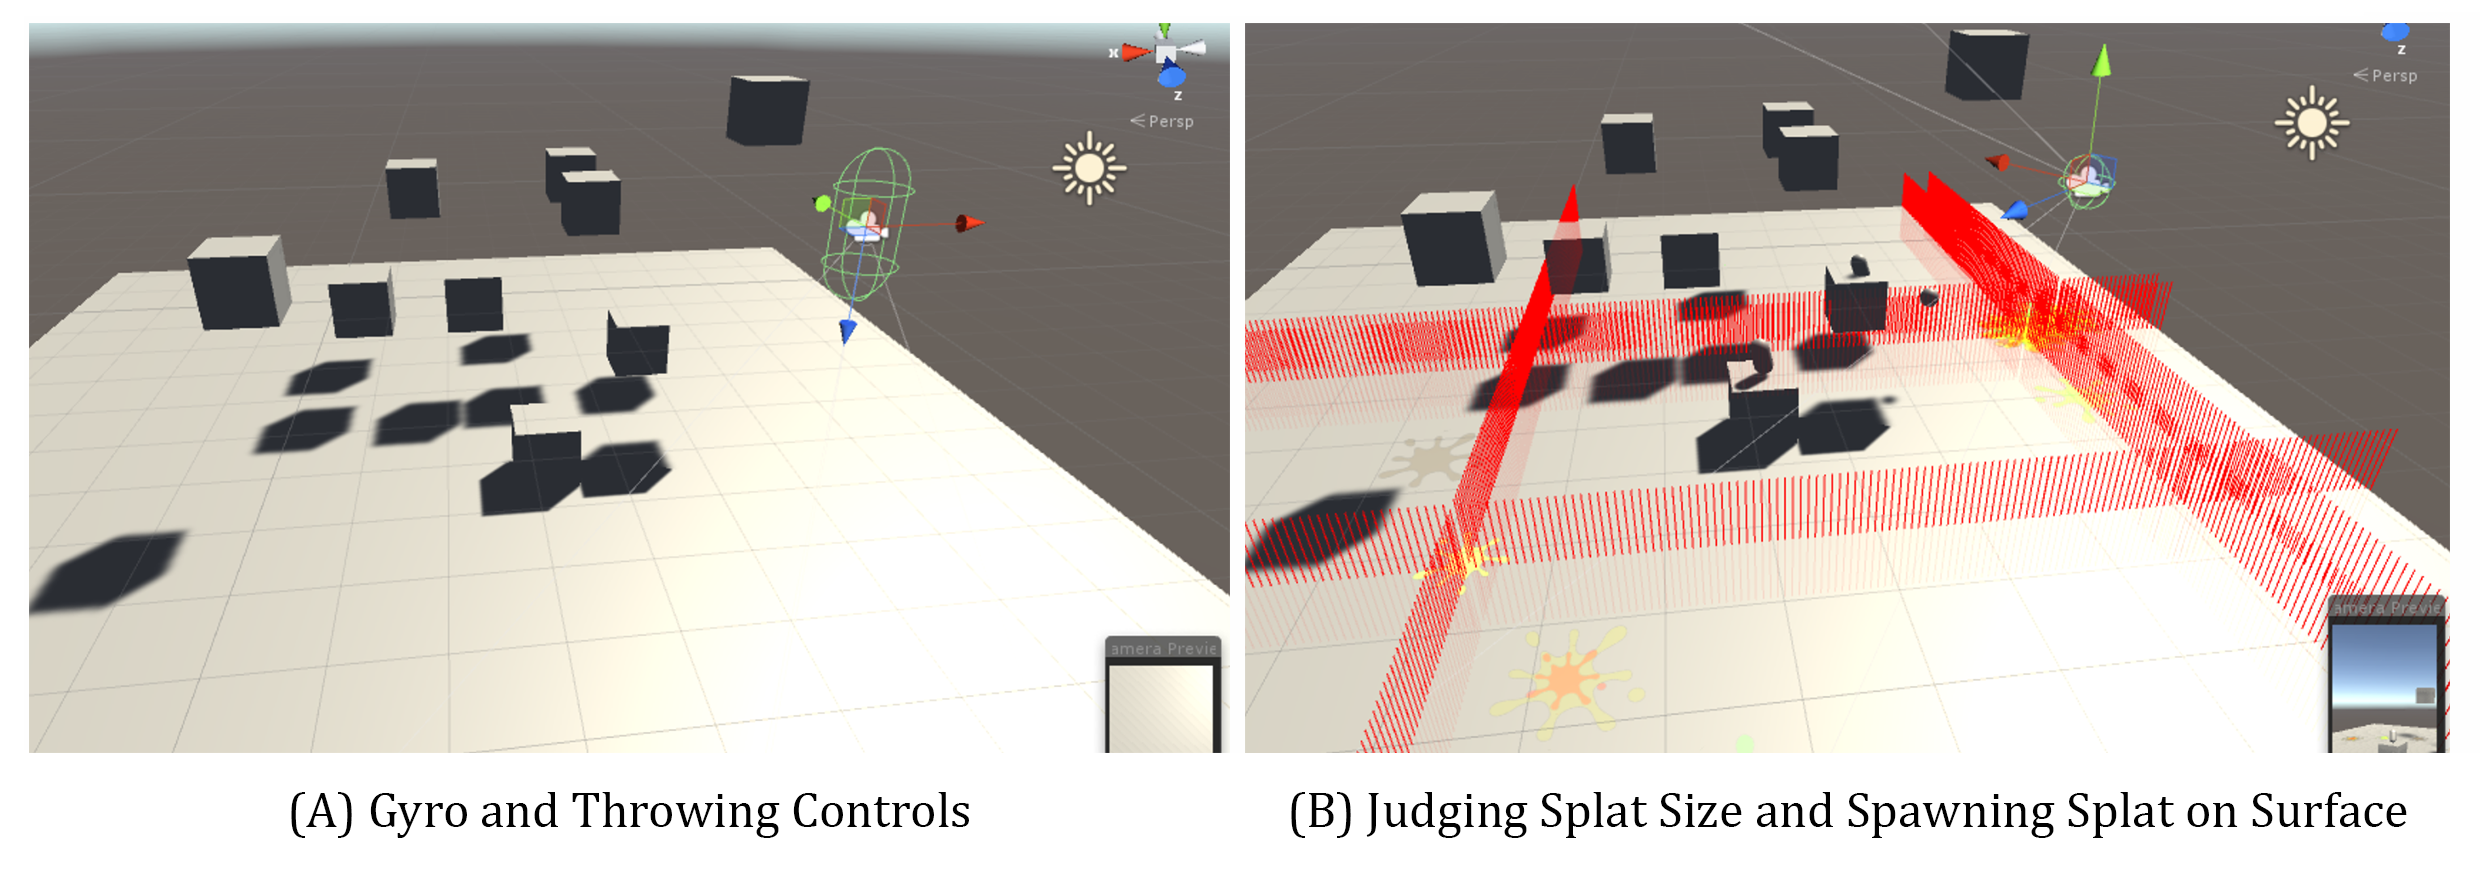
\includegraphics[width = \paperwidth]{Madkamp/TestScene}}
    \caption{The Test Level}
    \label{TestScene}
  \end{figure}
\end{center}

\begin{center}
  \begin{figure}
    \noindent\makebox[\textwidth]{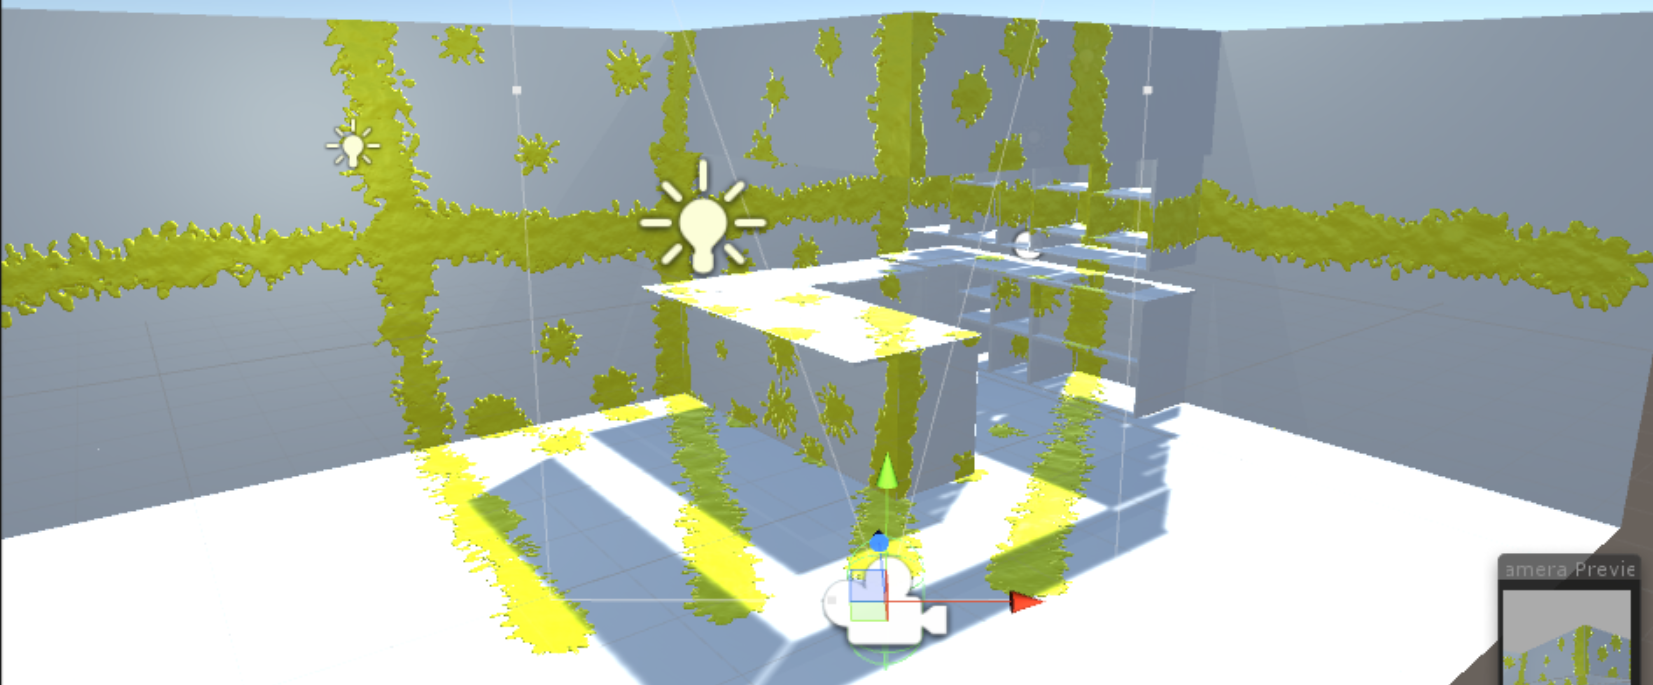
\includegraphics[width = \paperwidth]{Madkamp/UVSplat}}
    \caption{UV Mapping Splat Approach}
    \label{UVSplat}
  \end{figure}
\end{center}

The rest of the prototype was fairly simple. In the final level a placeholder for Torsten is set on a track around the kitchen and as soon the line of sight between Torsten and the player is unobstructed, Torsten will throw projectiles at the player in a predefined rhythm. To dodge Torsten's projectiles the player can look away from the approaching fruit or vegetable.

\subsubsection{Torstens Mund}
Torstens Mund, or \textit{Torsten's Mouth}, is a concept for a playful application. It is a playful application instead of a game because it does not contain any type of conflict and there is no quantifiable outcome of the play activity \cite[ch. 7, p. 11]{salen}. In Torstens Mund, the player is situated inside of Torsten's mouth and is able to look out through his open mouth. It is developed for mobile devices and utilises the built-in camera in such devices, so the world portrayed outside of the mouth is the real world as seen through the camera. When the player touches the device's screen Torsten starts chewing, on a still image of what was visible at the time of the input, and gives his impression of what that tastes like.

We initiated the work with a division of labour: The other intern would do art and animation and I would implement controls and mechanics. The first problem was how to integrate the camera feed into the prototype. This proved to be difficult mainly because it involved getting permissions, screen orientation and resolution from the device and obsolete documentation. Once I had the camera feed I needed to visualise it somehow. I did this by assigning it to the texture of an in-game object. The next challenge was to capture a still image and have the mouth chew on it. I figured that the simplest, possibly not best, solution, was to animate a simple rectangle to simulate the crumbling of something being chewed (see figure \ref{ChewAni}).

\begin{center}
  \begin{figure}
    \noindent\makebox[\textwidth]{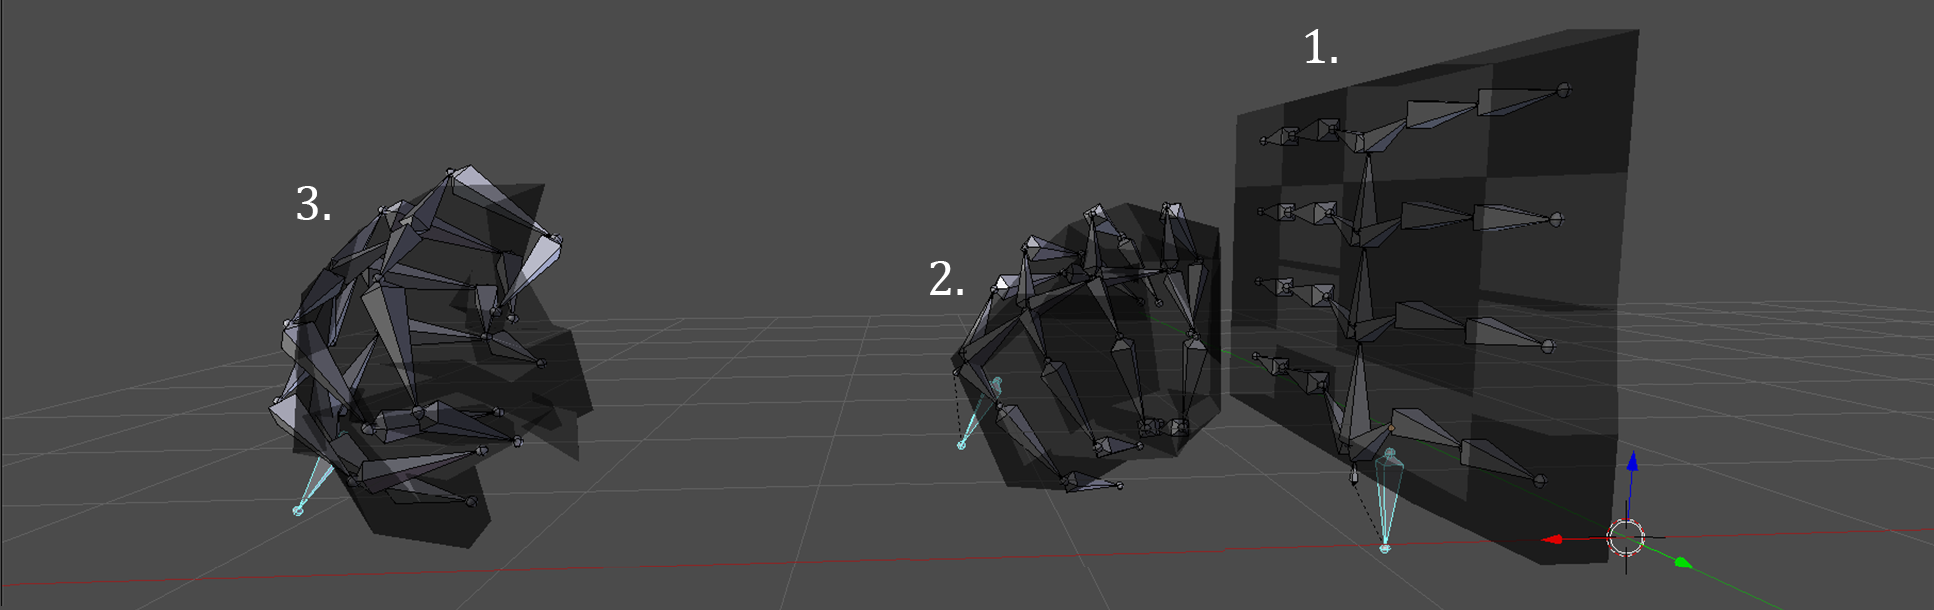
\includegraphics[width = \paperwidth]{TorstensMund/ChewAnimation}}
    \caption{The Animation Timeline of the Still Image being Chewed}
    \label{ChewAni}
  \end{figure}
\end{center}

The impression Torsten expresses after having chewed on something is based on the average colour of a square section of the centre of the still image. A random sound clip corresponding to the colour is then played. Examples of these follows:
\begin{itemize}
  \item Yellow: Ew, this tastes like pee.
  \item Blue: This tastes like jellyfish, or something like that.
  \item Brown: Pew, this tastes like sour underpants.
  \item Green: I like this, this tastes like a cucumber.
\end{itemize}
